\newpage
\subsection{PQR}

\textbf{Motivation.} During the initial research for a thesis subject, I came across \cite{dlchess:2014} which seemed an interesting approach to train a neural network to evaluate positions. Since it was released in 2014, it predates the NNUE era and the training data was suboptimal (Lichess database \cite{lichessdb} with human moves). So I decided to try to replicate the idea using modern datasets, better moves and a proper engine. The \enquote{PQR} method itself was explained in detail in the previous chapter.  Remember that $p$ is a position in the dataset, $q$ is the position obtained by making the best move according to the dataset and $r$ is a random position obtained making a random move from $p$ such that $r \neq q$. \\

Before starting the experiment, I checked if existing networks trained with the conventional method behave under the principles of the PQR method: ${f(p) = -f(q)}$ and ${f(r) > f(q)}$. In the left plot of figure \ref{pqr-eval}, we can see that values of $f(p)$ and $f(q)$ are negatively correlated, which supports the principle that $f(p)=-f(q)$. In the right plot, we can see that the distribution of the difference between $f(r)$ and $f(q)$ is mostly positive, which supports the principle that $f(r) > f(q)$. This shows that the principles that the PQR method relies on are properties that manifest in existing models.

\begin{figure}[H]
\centering
\makebox[\textwidth]{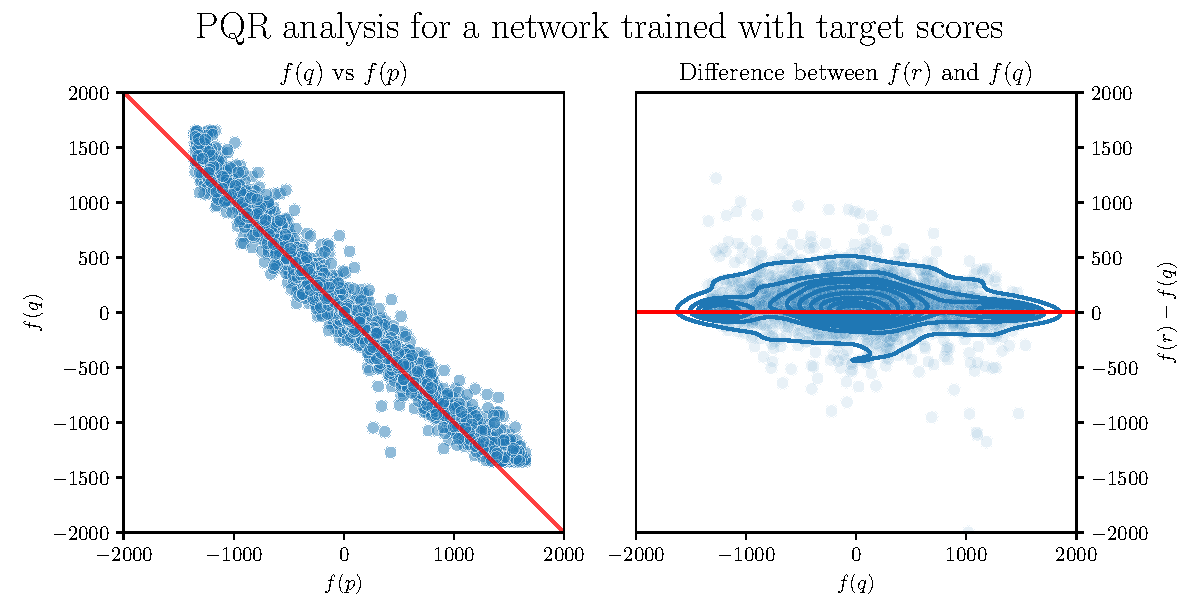
\includegraphics[width=\textwidth]{./dynamic/output/pqr_eval.pdf}}
\caption{Analysis of $N=4000$ PQR positions using a model trained with target scores and the feature set \featureset{All}.}
\label{pqr-eval}
\end{figure}

\textbf{Experiment.} I will train the canonical \featureset{All} feature set with this method in two ways:

\begin{itemize}
\item \textbf{Train from scratch.} The network is initialized with random weights and trained with the PQR method. This is what the original authors did, and I do not expect to reach the performance of models trained with the evaluations method. Using precomputed evaluations as a target is a lot simpler for the model, since it only has to learn to mimic the scores.

\item \textbf{Train from a checkpoint.} A strong checkpoint trained with the other method is used to initialize the network. This way, the network does not have to learn too much at once and may enable it to improve the existing parameters. I believe that two scenarios are likely to happen: the model improves very slowly, or it completely forgets what it have learned before and ends up like a model trained from scratch. The best scenario is that the model improves slowly, proving that it can be used to further optimize existing models.
\end{itemize}

The training data is not filtered the same way as with target scores, where it was known that captures and checks are detrimental. When choosing a random position $R$ from a position $P$, the number of available moves to choose from is $m$ (including $P \rightarrow Q$). A training sample is skipped if $m < M$. The reasoning behind $M$ is that the bigger the pool to choose from, the more likely it is to find a move that is worse than $P \rightarrow Q$. Note that $M \geq 2$ since otherwise there is only one available move.

Choosing fixed values of $M$ is not ideal, since the number of available moves varies throughout the game. A value of $M$ will be chosen for every turn in the game, based on the distribution of available moves for that particular turn and color. It is known that the white player has more available moves in average than the black player, so $M$ will be different for each.

Four networks will be trained from scratch where $M$ is chosen to filter 0\%, 25\%, 50\% and 75\% of samples with the least available moves for that turn. In figure \ref{avg-moves} we can see the value of $M$ changing throughout the game for each percentile. Note that when $p=0$ the value of $M$ is 2 in every turn, so no filtering is done. \\

\begin{figure}[H]
\centering
\makebox[\textwidth]{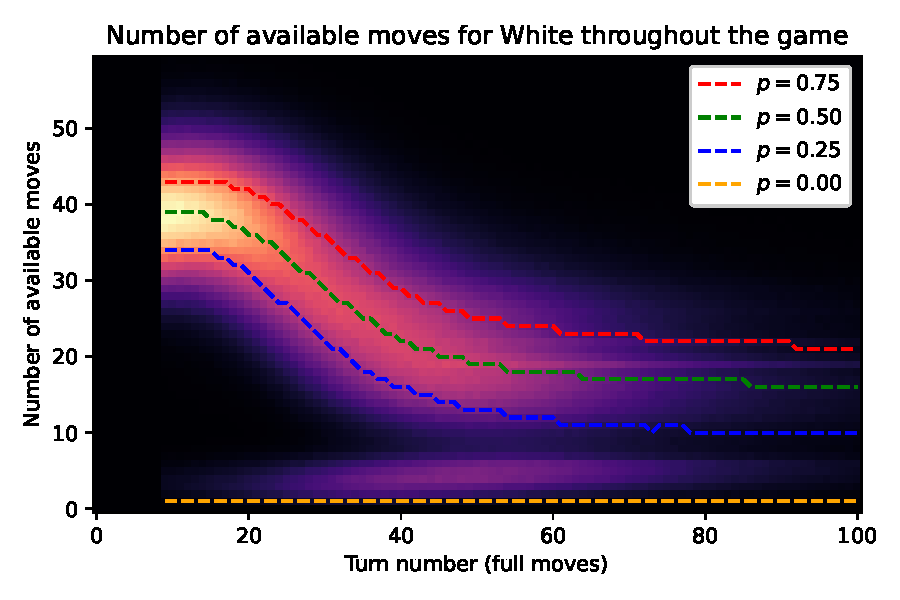
\includegraphics[width=\textwidth]{./dynamic/output/avg_moves.pdf}}
\caption{Heatmap showing the number of available moves for white throughout 100 turns (full moves). The color gradient indicates the density of occurrences in the dataset (N=25M) for positions with a certain number of available moves in a given turn. The plot for black is not shown because it is very similar.}
\label{avg-moves}
\end{figure}

\textbf{Results.} asd


% After training a single network from scratch, the results do not look promising. Looking at figure \ref{pqr1-evolution}, we can see that the network improves steadily up to the epoch 32 (trained on 3.2 billion samples), but then it starts to get consistently worse. There are no indications of overfitting, as the validation loss is still decreasing.

\begin{figure}[H]
\centering
\makebox[\textwidth]{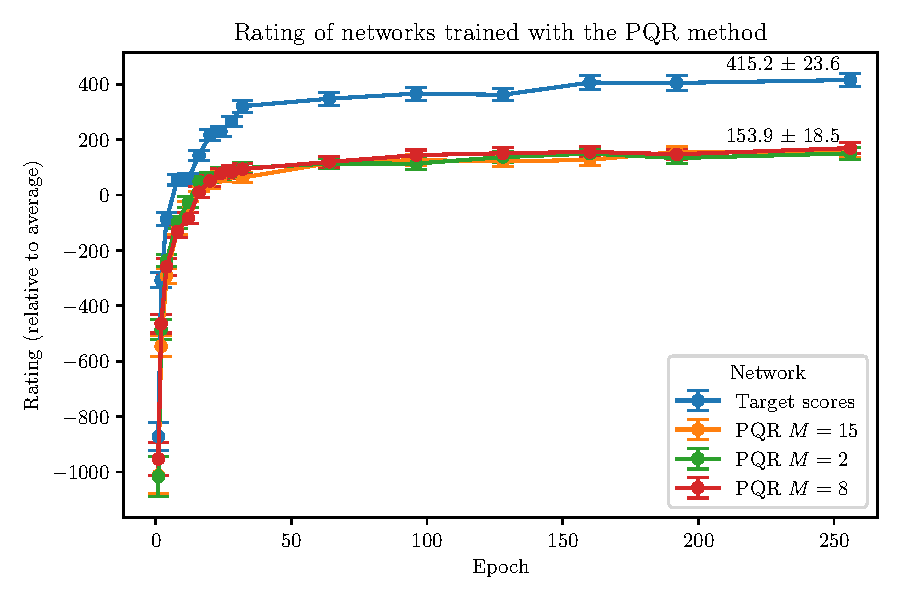
\includegraphics[width=\textwidth]{./dynamic/output/pqr_comparison.pdf}}
\caption{Rating evolution of a network trained with the PQR method from scratch.}
\label{pqr1-evolution}
\end{figure}

To investigate, I tried comparing the loss of 

. \\

seguir...

Positions that are very similar in score f(q)~f(r) are being penalized the same way that more extreme ones. A way to mitigate this is generate a dataset which takes into account multiple lines of play, and only include samples where there is a significant difference between the moves.


% Initially, the loss proposed was going to work in score-space with the proper scaling without going through the transformation to WDL-space, however the network was 

The most important decision is how the random position is chosen.

----

Further work:

* change the filter on the minimum number of moves to draw during training
* lines of play
* data with more depth
* possibly detect zugzwang positions

---
* try to change dataset to filter out similar f(q) and f(r) scores
* try to give a good distribution of those
* end up again with scores, because they contain all that information
